\documentclass[9pt]{beamer}
\usetheme{boxes}
\usetheme{Boadilla}
\usecolortheme{beaver}
%\usecolortheme{sidebartab}
% \usefonttheme{structurebold}
\usefonttheme{serif}



\usepackage{etex}
% \usepackage{helvet}
%\usepackage{asymptote}


% \usepackage{helvet}
\usepackage{amsmath, amssymb}
\usepackage{color}
%\usepackage{asymptote}
\usepackage{mathrsfs}
\usepackage{dsfont}
\usepackage{url}
\usepackage{cancel}
\usepackage{tikz}
\usetikzlibrary{fit,positioning}
\usetikzlibrary{shapes,matrix,decorations.markings,arrows}
\usetikzlibrary{graphs}

\usepackage{pst-sigsys,pst-plot,pstricks-add}
%\usepackage{auto-pst-pdf}
\usepackage{pst-pdf}

\usepackage{bbm}
\def\ind{\mathbbm{1}} %Indicator function

%
%
%\newcommand{\LABEQ}[1]{\label{eq:#1}}%\mathtt{[eq:#1]}\qquad
%\newcommand{\LABALG}[1]{\label{alg:#1}}%\mathtt{[lab:#1]}\qquad
%\newcommand{\LABTAB}[1]{\label{tab:#1}}%{\tt [tab:$\text{$#1$}$]}}
%\newcommand{\LABFIG}[1]{\label{fig:#1}}%{\tt [fig:$\text{$#1$}$]}}
%\newcommand{\LABTHM}[1]{\label{thm:#1}}%{\tt [thm:#1]}}
%\newcommand{\LABPRP}[1]{\label{prp:#1}}%{\tt [prp:#1]}}
%\newcommand{\LABLEM}[1]{\label{lem:#1}}%{\tt [lem:#1]}}
%\newcommand{\LABCOR}[1]{\label{cor:#1}}%{\tt [cor:#1]}}
%\newcommand{\LABDFN}[1]{\label{dfn:#1}}%{\tt [dfn:#1]}}
%\newcommand{\LABFNT}[1]{\label{fnt:#1}}%{\tt [fnt:#1]}}
%\newcommand{\EQ}[1]{\eqref{eq:#1}}%$^{\text{\tt [#1]}}$} %used to be  %{(\ref{eq:#1})}
%\newcommand{\ALG}[1]{~\ref{alg:#1}}
%\newcommand{\TAB}[1]{~\ref{tab:#1}}%$^{\text{\tt [#1]}}$}
%\newcommand{\FIG}[1]{\ref{fig:#1}} %$^{\text{\tt [#1]}}$}
%\newcommand{\THM}[1]{~\ref{thm:#1}}%$^{\text{\tt [#1]}}$}
%\newcommand{\COR}[1]{~\ref{cor:#1}}%$^{\text{\tt [#1]}}$}
%\newcommand{\PRP}[1]{~\ref{prp:#1}}%$^{\text{\tt [#1]}}$}
%\newcommand{\LEM}[1]{~\ref{lem:#1}}%$^{\text{\tt [#1]}}$}
%\newcommand{\DFN}[1]{~\ref{dfn:#1}}%$^{\text{\tt [#1]}}$}
%\newcommand{\FNT}[1]{~\ref{fnt:#1}}%$^{\text{\tt [#1]}}$}
%\newcommand{\PAGEEQ}[1]{~\pageref{eq:#1}}
%\newcommand{\PAGETAB}[1]{~\pageref{tab:#1}}
%\newcommand{\PAGEFIG}[1]{~\pageref{fig:#1}}
%\newcommand{\LABCHAP}[1]{\label{chap:#1}}%{\tt [chap:#1]}}
%\newcommand{\LABSEC}[1]{\label{sec:#1}}%{\tt [sec:#1]}}
%\newcommand{\LABSSEC}[1]{\label{ssec:#1}}%{\tt [ssec:#1]}}
%\newcommand{\LABSSSEC}[1]{\label{sssec:#1}}%{\tt [sssec:#1]}}
%\newcommand{\CHAP}[1]{~\ref{chap:#1}}%$^{\text{\tt [c:#1]}}$}
%\newcommand{\SEC}[1]{~\ref{sec:#1}}%$^{\text{\tt [s:#1]}}$}
%\newcommand{\SSEC}[1]{~\ref{ssec:#1}}%$^{\text{\tt [ss:#1]}}$}
%\newcommand{\SSSEC}[1]{~\ref{sssec:#1}}%$^{\text{\tt [sss:#1]}}$}
%
\definecolor{darkblue}{rgb}{0.0, 0.0, 0.45}
\setbeamercolor{title}{fg=darkblue}
\setbeamercolor{frametitle}{fg=darkblue}
\newcommand{\myitem}{\item[$\bullet$]}

%gets rid of bottom navigation bars
\setbeamertemplate{footline}[page number]{}

%gets rid of navigation symbols
\setbeamertemplate{navigation symbols}{}


\newcommand{\ve}[1]{\boldsymbol{#1}}
\def\X{\ve{X}}
\def\x{\ve{x}}
\def\s{\ve{s}}
\def\S{\ve{S}}
\def\hx{\hat{\x}}
\def\m{\ve{m}}
\def\y{\ve{y}}
\def\G{\ve{G}}
\def\H{\ve{H}}
\def\C{\mathcal{C}}
\def\O{\mathcal{O}}
\def\b{\ve{b}}
\def\E{\mc{E}}

\def\k{{\mathtt{k}}}

\def\pe{{\varepsilon}}
\def\n{{\mathtt{n}}}
\def\nn{{\nonumber}}
\def\rate{{\mathtt{r}}}


%Original left degree distribution
\def\lambimax{{l_{\text{max}}}}				       %maximun lambda degree
\newcommand{{\Tlmax}}[1]{\lambimax(#1)}      %maximun left degree  (t)
\newcommand{\lambi}[1]{\lambda_{#1}}		%lambda_i
\newcommand{\lamb}[1]{\lambda(#1)}		%lambda(x),lambda(t)
\def\lambfull{{\lamb{x}=\sum_{i=1}^{\lambimax}\lambi{i}x^{i-1}}} %Full expression of lambda(x)
\def\lavg{{l_{\text{avg}}}}						%lavg
\newcommand{\lav}[1]{\lavg(#1)}			%lavg(t)

%Original right degree distribution
\def\rhimax{{r_{\text{max}}}}
\newcommand{\rhi}[1]{\rho_{#1}}
\newcommand{\rh}[1]{\rho(#1)}
\def\rhofull{{\rh{x}=\sum_{j=1}^{\rhimax}\rhi{j}x^{j-1}}}
\def\ravg{{r_{\text{avg}}}}
\newcommand{\rav}[1]{\ravg(#1)}



\newcommand{\mc}[1]{\mathcal{#1}}
\def\sX{\mc{X}}
\def\N{\mc{N}}
\newcommand{\mxf}[3]{m^{#3}_{X_{#1}\rightarrow f_{#2}}(x_{#1})}
\newcommand{\mfx}[3]{m^{#3}_{f_{#2}\rightarrow X_{#1}}(x_{#1})}

\newcommand\Def[1]{{\textbf{\textcolor{DeepSkyBlue4}{Definition:}}\\\emph{#1}\\\begin{center} \textcolor{DeepSkyBlue4}{------------------------} \end{center}}}
\newcommand\Prop[1]{{\textbf{\textcolor{red}{Property:}}\\\emph{#1}\\\begin{center} \textcolor{red}{------------------------} \end{center}}}



\newcommand{\fs}[2]{#2}

\title[]{BP decoding of LDPC codes}
\author[\textcolor{white}{Advanced Digital Communications}]{Introduction to Graphical Models and Inference for Communications\\\vspace*{3mm}{\small \textcolor{black}{UC3M}}
}
%\date[08/02/2016]{{08/02/2016}}
\institute{\textcolor{white}{}}

% \pgfdeclareimage[height=0.5cm]{ITW}{pics/Logo.png}
%  \logo{\pgfuseimage{ITW}}

\AtBeginSection[]
{
  \begin{frame}<beamer>{Index}
    \tableofcontents[currentsection,currentsubsection]
  \end{frame}
}

\begin{document}

\frame{
\titlepage
\thispagestyle{empty}
\begin{center}

\includegraphics[scale=0.05]{Figuras/uc3m-logo.pdf}
\end{center}
}



%\section{LDPC codes over the Gaussian channel}

\frame{

%\begin{center}
%\begin{pspicture}[](8,2)
%   \pssignal(-1,1){x}{$S\in\{\pm 1\}$}
%   \pscircleop(2,1){oplus}
%   \pssignal(5,1){y}{$Y\sim\mathcal{N}(S,\sigma^2)$}
%   \pssignal(2,2){z}{$Z\sim\mathcal{N}(0,\sigma^2)$}	
%    \pssignal(8,1){snr}{$SNR=1/\sigma^2$}	
%   %-----------------
%   \psset{arrows=->}
%   \ncline{x}{oplus}  \ncline{oplus}{y}  \ncline{z}{oplus}
%\end{pspicture}

\frametitle{Binary-input discrete AWGN (BIAWGN) channel }
\begin{figure}[!ht]
\centering
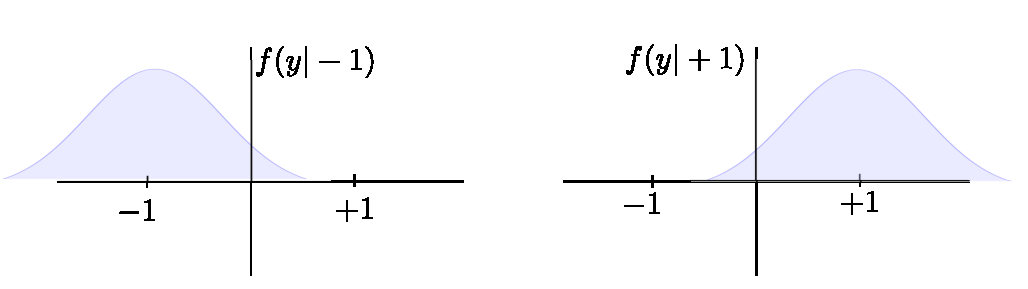
\includegraphics[scale=0.6]{Gauss4.pdf}
\end{figure}
%\end{center}



\begin{block}{}
%\begin{align*}
%P(S=\sqrt{E_b}|y)&=\frac{p(y|\sqrt{E_b})P(s=\sqrt{E_b})}{p(y|\sqrt{E_b})P(S=\sqrt{E_b})+p(y|-\sqrt{E_b})P(S=\sqrt{-E_b})}
%\end{align*}
Assuming a uniform prior distribution $P(S=1)=P(S=-1)=\frac{1}{2}$...
\begin{align*}
P(S=1|y)&=\frac{f(y|1)}{f(y|1)+f(y|-1))}
\end{align*}
\end{block}


}

\frame{
\frametitle{Optimal decoder for the BIAWGN channel}
\begin{itemize}
\item LDPC codeword of $\n$ bits.  
\begin{align*}
\ve{s}&=(\begin{array}{cccc} s_1 & s_2 & \ldots & s_\n\end{array})\qquad \text{Vector of $\n$ encoded BPSK symbols}.
\\
\y&=(\begin{array}{cccc} y_1 & y_2 & \ldots & y_\n\end{array})\qquad \text{Observation vector}.
\end{align*}
\end{itemize}

\begin{itemize}
%\item A priori probabilities ignore dependencies between coded bits: $p(s[n]|y[n])$ for $n=1,\ldots, N$.
\item \textbf{Optimal LDPC decoder: bitwise-MAP decoder.}  For $i=1\ldots,n$, 
\begin{enumerate}
\item Compute 
\begin{align*}
P(S_i=+1| \y) 
\end{align*}
\item If $P(S_i=+1| \y) > 0.5$, then $\hat{S}_i=1$.
\end{enumerate}
\end{itemize}
}

\frame{

\begin{alertblock}{Baye's rule ...}
\begin{align*}
P(\S=\s|\y)&=\frac{f(\y|\s)P(\S=\s)}{f(\y)}, \quad P(\S=\s)=\frac{1}{2^{\rate \n}}\quad  \forall \s\in\mathcal{C},\qquad f(\y|\s)=\prod_{j=1}^{\n}f(y_j|s_j)
\end{align*}
\end{alertblock}

}


\frame{
\begin{alertblock}{}
\begin{align*}
P(\S=\s|\y)&=\frac{f(\y|\s)P(\S=\s)}{f(\y)}, \quad P(\S=\s)=\frac{1}{2^{\rate \n}}\quad  \forall \s\in\mathcal{C},\qquad f(\y|\s)=\prod_{j=1}^{\n}f(y_j|s_j)
\end{align*}
\end{alertblock}

Therefore ....
\begin{align*}
P(S_i=1| \y)&=\sum_{\substack{\ve{s}\in\mathcal{C}: s_i=1}}P(\S=\s|\y)\\
&=\frac{1}{f(\y)}\frac{1}{2^{\rate \n}}\sum_{\substack{\ve{s}\in\mathcal{C}: s_i=1} } ~\prod_{j=1}^{\n} f(y_j|s_j)
\\ &\propto \sum_{\substack{\ve{s}\in\mathcal{C}: s_i=1} } ~\prod_{j=1}^{\n} f(y_j|s_j)
\end{align*}
}



\frame{
\frametitle{Optimal decoder for the BIAWGN channel}

\begin{exampleblock}{}
\begin{align*}
P(S_i=1| \y)\propto \sum_{\substack{\ve{s}\in\mathcal{C}: s_i=1} } ~\prod_{j=1}^{\n} f(y_j|s_j) \qquad 
P(S_i=-1| \y)\propto \sum_{\substack{\ve{s}\in\mathcal{C}: s_i=-1} } ~\prod_{j=1}^{\n} f(y_j|s_j)
\end{align*}
\end{exampleblock}


\begin{itemize}
\item The number of terms to be sum is roughly half of the codewords $2^{\rate \n-1}$.
\item The decoding complexity grows exponentially fast with $\n$.
\item Prohibitive complexity for $\n\geq 100$!!
\end{itemize}
}


%\frame{
%\frametitle{Optimal decoder for the BIAWGN channel}
%\begin{block}{Rate $\rate$ and code length $N$}
%\begin{align*}
%p(s[n]=1\Big| \y)=\frac{1}{2^{\rate N}}\underbrace{\sum_{\substack{\ve{s}\in\mathcal{C}: s[n]=1} } ~~\overbrace{\prod_{i=1}^{N} p(s[i]|y[i])}^{\text{A priori probability codeword $\ve{s}$}}}_{\text{All codewords for which $s[n]=1$}}
%\end{align*}
%\end{block}
%
%\begin{itemize}
%\item The number of terms to be sum is roughly half of the codewords $2^{\rate N-1}$.
%\item The decoding complexity grows exponentially fast with $N$.
%\item Prohibitive complexity for $N\geq 100$!!
%\end{itemize}
%}




\frame{
\frametitle{Approximate decoder for the BIAWGN channel}

\begin{itemize}
\item Belief Propagation (BP) algorithm to approximate marginals!
\item Message-Passing description.
\item Complexity grows linearly with the code length $\n$!
\item At each iteration, variable nodes in the Tanner graph send a ``belief" (estimated probability) to check nodes and check nodes recompute a belief for each variable node.
\item We proceed in this way for a given number of iterations $\ell_{\max}$.
\item The associated factor graph is sparse, only contains very large cycles involving a large number of variables. 
\item BP estimates, based on local computations, are reasonably accurate.
\end{itemize}
%
%\vspace{0.5cm}
%\begin{center}
%\begin{tikzpicture}[scale=0.6]
%\tikzstyle{factor}=[rectangle, thick, draw =black,fill=black, minimum size=0.4 cm]
%\tikzstyle{var}=[circle, thick, draw =black,fill=black,minimum size=0.4 cm]
%\tikzstyle{connect}=[-latex, thick]
%
%
%	\node[var] (x_1) at (-1,0) []{};
%	\node[var] (x_2) at (1,0) []{};
%	\node[var] (x_3) at (3,0) []{};
%	\node[var] (x_4) at (5,0) []{};
%	\node[var] (x_5) at (7,0) []{};
%	\node[var] (x_6) at (9,0) []{};
%	\node[var] (x_7) at (11,0) []{};
%	
%	
%	\node[factor] (c_1) at (3,-3) []{};
%	\node[factor] (c_2) at (5,-3) []{};
%	\node[factor] (c_3) at (7,-3) []{};
%	
%	\node[] at (5, 1) {Variable Nodes};
%	\node[] at (5, -4) {Check Nodes};
%	
%	\path
%	 (x_1) edge[] (c_1)
%	 (x_2) edge[] (c_2)
%	 (x_3) edge[] (c_1)
%	 (x_3) edge[] (c_2)
%	 (x_4) edge[] (c_3)
%	 (x_5) edge[] (c_1)
%	 (x_5) edge[] (c_3)
%	 (x_6) edge[] (c_2)
%	(x_6) edge[] (c_3)
%	(x_7) edge[] (c_1)
%	(x_7) edge[] (c_2)
%	(x_7) edge[] (c_3);
%
%\end{tikzpicture}
%\end{center}
%
}

\frame{
\frametitle{Towards a BP formulation}

\begin{align*}
P(S_i=1| \y)&\propto \sum_{\substack{\ve{s}\in\mathcal{C}: s_i=1} } ~\prod_{j=1}^{\n} f(y_j|s_j)\\
&=\sum_{\substack{\ve{s}\in\{0,1\}^n: s_i=1} } \prod_{j=1}^{\n} f(y_j|s_j)  \ind[\H\x=\ve{0}~~\text{(mod 2)}]
\end{align*}

\begin{itemize}
\item $\ind[\H\x=\ve{0}~~\text{(mod 2)}]$ can be decomposed as follows
\begin{align*}
\prod_{q=1}^{\k} \ind[\ve{h}_q \x=0]
\end{align*}
where $\ve{h}_q$ is the $q$-th row of $\H$ and $\k$ is the number of rows.
\end{itemize}

\begin{block}{}
\begin{align*}
P(S_i=1| \y)\propto \sum_{\substack{\ve{s}\in\{0,1\}^n: s_i=1} } \prod_{j=1}^{\n} f(y_j|s_j)   \prod_{q=1}^{\k} \ind[\ve{h}_q \x=0]
\end{align*}
\end{block}
}

\frame{
\frametitle{The LDPC Tanner graph}
\begin{align*}
P(\S=\s|\y)\propto \prod_{j=1}^{\n} f(y_j|s_j)   \prod_{q=1}^{\k} \ind[\ve{h}_q \x=0]
\end{align*}

\vspace{0.5cm}

\begin{center}
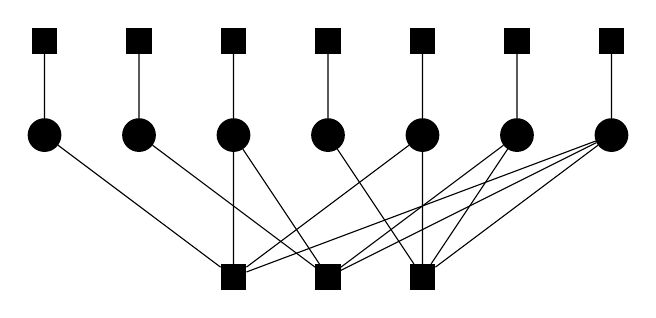
\begin{tikzpicture}[scale=0.6]
\tikzstyle{factor}=[rectangle, thick, draw =black,fill=black, minimum size=0.3 cm]
\tikzstyle{var}=[circle, thick, draw =black,fill=black,minimum size=0.4 cm]
\tikzstyle{connect}=[-latex, thick]


	\node[var] (x_1) at (-1,0) []{};
	\node[var] (x_2) at (1,0) []{};
	\node[var] (x_3) at (3,0) []{};
	\node[var] (x_4) at (5,0) []{};
	\node[var] (x_5) at (7,0) []{};
	\node[var] (x_6) at (9,0) []{};
	\node[var] (x_7) at (11,0) []{};
	
	
	\node[factor] (cx_1) at (-1,2) []{};
	\node[factor] (cx_2) at (1,2) []{};
	\node[factor] (cx_3) at (3,2) []{};
	\node[factor] (cx_4) at (5,2) []{};
	\node[factor] (cx_5) at (7,2) []{};
	\node[factor] (cx_6) at (9,2) []{};
	\node[factor] (cx_7) at (11,2) []{};
	
	\node[factor] (c_1) at (3,-3) []{};
	\node[factor] (c_2) at (5,-3) []{};
	\node[factor] (c_3) at (7,-3) []{};
	
	
	
	\path
	 (cx_1) edge[] (x_1)
	  (cx_2) edge[] (x_2)
	  (cx_3) edge[] (x_3)
	  (cx_4) edge[] (x_4)
	  (cx_5) edge[] (x_5)
	  (cx_6) edge[] (x_6)  
	 (cx_7) edge[] (x_7)
	 (x_1) edge[] (c_1)
	 (x_2) edge[] (c_2)
	 (x_3) edge[] (c_1)
	 (x_3) edge[] (c_2)
	 (x_4) edge[] (c_3)
	 (x_5) edge[] (c_1)
	 (x_5) edge[] (c_3)
	 (x_6) edge[] (c_2)
	(x_6) edge[] (c_3)
	(x_7) edge[] (c_1)
	(x_7) edge[] (c_2)
	(x_7) edge[] (c_3);

\end{tikzpicture}
\end{center}

From here you already know how to implement a BP decoder.
}

\frame{
\frametitle{Excersise}

Show that the BP message passing rules for binary LDPC codes can be simplified to the following experessions.

\begin{block}{Update rule at variable nodes}
Variable with $K+1$ neighbours sends a message to neighbour K+1:
\begin{align*}
l_{K+1}=\sum_{k=1}^{K} l_k,
\end{align*}
where $l_j$, $j=1,\ldots,K+1$ are real scalars. 
\end{block}

\begin{block}{Update rule at parity check nodes}
Factor with $J+1$ neighbours sends a message to neighbour J+1:
\begin{align*}
l_{J+1}= 2\text{tanh}^{-1}\left(\prod_{j=1}^{J}\tanh(l_j/2)\right)
\end{align*}
where $l_j$, $j=1,\ldots,J+1$ are real scalars. 
\end{block}

}


\end{document}

